\section{Introduction}
\seclabel{extended-abstract}

Robots in warehouse order fullfillment and small- to medium-scale manufacturing must be able to efficiently grasp and manipulate new products and parts.
For example, a robot processing orders in a distribution warehouse must quickly plan graps for new consumer products to place them in shipping containers. 
% Above motivates speed and adaptivity
% Statement motivating robustness to uncertainty
Furthermore, a robot may not fully observe the state of the workspace, such as the pose or frictional properties of consumer products, due to sensor imprecision and missing data resulting from occlusions.
This poses a challenge for grasp planning with either analytic methods~\cite{ferrari1992, ciocarlie2009} that require precise knowledge of contact locations and surface normals or data-driven approaches~\cite{bohg2014data} that attempt to build a statistical model of grasp success over the massive number of configurations of the environment.
%This motivates an approach to grasp planning that is fast, robust to uncertainty about the state of the robot and environment, and can adapt to new objects and perturbations in the envrionment.

Past work has attempted to overcome this by planning grasps analytically with high probability of force closure~\cite{kehoe2012toward, kim2012physically, laskey2015bandits, mahler2015gp, weisz2012pose}, or using data-driven methods to predict grasp success from human labels~\cite{balasubramanian2012physical, detry2013learning,  herzog2014learning, kappler2015leveraging, lenz2015deep, saxena2008robotic} or empirical successes on a physical robot~\cite{boularias2014efficient, brook2011collaborative, detry2011learning, kroemer2010combining, montesano2012active}.
Many works on grasp selection with probablity of force closure evaluate a set of candidate grasps using sampling and select the highest quality grasp either using brute force sampling~\cite{kehoe2012toward, kim2012physically, weisz2012pose}, iterative pruning~\cite{kehoe2012estimating}, or Multi-Armed Bandit (MAB) algorithms to adaptively sample more promising grasps~\cite{barto1998reinforcement,
lai1985asymptotically, laskey2015bandits, robbins1985some}.
However, MAB algorithms, the current fastest sampling method, still required approximately 10 samples per grasp to converge to a solution and needed to be re-run for every new object.

On the other hand, data-driven approaches have shown promise over analytic methods on physical robot trials~\cite{balasubramanian2012physical, herzog2014learning} possibly due to a reduction in modelling error.
The number of objects and grasps tested is typically on the order of tens to hundreds for physical robot trials and at most a few thousand objects and hundreds of thousands of grasps when using simulation or human labels~\cite{goldfeder2009columbia, lenz2015deep, kappler2015leveraging}.
In comparison, state-of-the-art learning results in image classification~\cite{deng2009imagenet, krizhevsky2012imagenet} and speech recognition~\cite{cieri2004fisher, hannun2014deepspeech} relied on datasets containing tens of millions of examples.
This raises the question: will maching learning for grasp planning under vast numbers of possible object poses, object shapes, environment configurations, etc., exhibit scaling effects similar to those observed in computer vision and speech recognition?
%may require orders of magnitude more data than in use currently.

%This motivated gradient-based methods based on approximations to the probabliity of force closure~\cite{mahler2015gp} and using Multi-Armed Bandit algorithms to adaptively sample more promising grasps~\cite{laskey2015bandits}, which reduced the number of samples until convregence by 10$\times$.
%However, the number of iterations was still prohibitively high for real-time execution and prior knowledge could not be utilized for new objects.

To make progress toward answering this question, we introduce the Dexterity Network (DexNet) 1.0, a dataset of tens of thousands of 3D mesh models and a system for building statistical models that predict grasp quality across the dataset.
DexNet is composed of laser-scanned 3D mesh models from the KIT object database~\cite{kasper2012kit}, the Amazon Picking Challenge objects, BigBIRD~\cite{singh2014bigbird}, and YCB ~\cite{calli2015benchmarking}, and synthetic 3D mesh models from 3DNet~\cite{wohlkinger20123dnet} and the SHREC 2014 large scale object retrieval challenge~\cite{li2015comparison}.
~\figref{dexnet-teaser} shows a subset of the objects in the dataset.
To measure similarity between objects, we form an object network based on Deep Convolutional Neural Networks (CNNs) trained to predict object categories from synthetic rendered images of each object~\cite{aubry2015understanding, li2015comparison}.
The DexNet system uses Google Compute Engine to launch up to 600 instances at a time for evaluating grasp quality on subsets of objects and takes approximately 9.5 hours to run 1,800 objects on 180 instances.

\begin{figure}[t!]
\centering
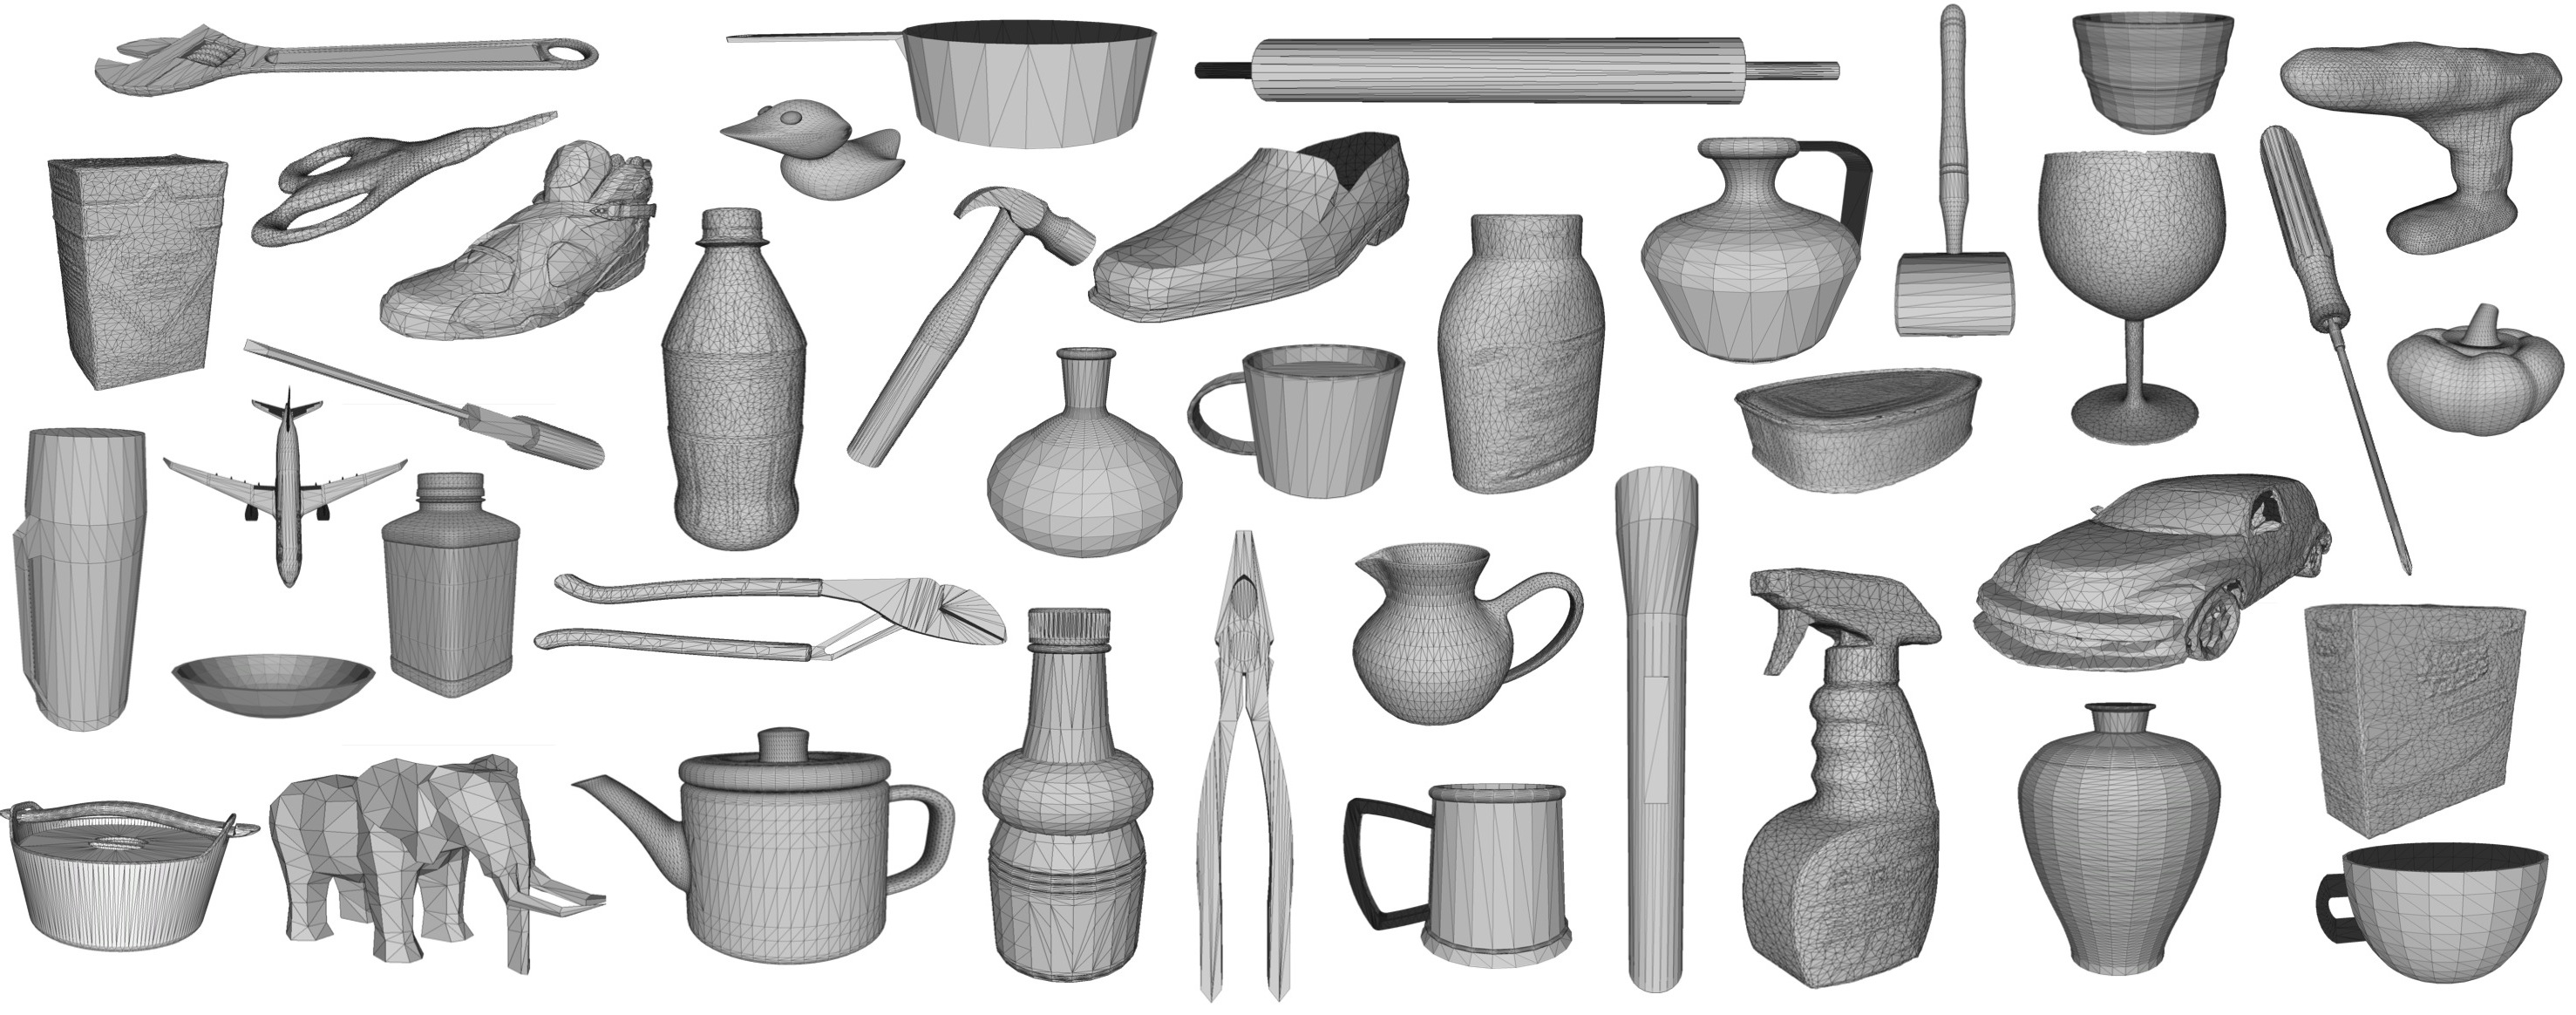
\includegraphics[scale=0.085]{figures/dexnet_collage.jpg}
\caption{Sample of 3D mesh models from the DexNet dataset. The dataset consists of over 30,000 models from laser-scanned datsets such as the KIT object database~\cite{kasper2012kit} and the Yale-CMU-Berkeley object set~\cite{calli2015benchmarking}, and synthetic datasets such as 3DNet\cite{wohlkinger20123dnet} and the SHREC 2014 object retrieval challenge dataset~\cite{li2015comparison} }
\figlabel{dexnet-teaser}
\vspace*{-15pt}
\end{figure}

In this work, we use DexNet to study the number of samples that MAB algorithms take to converge to a grasp with high probability of force closure across orders of magnitude of prior data of grasps with known quality.
To do so, we extend the MAB framework of Laskey et al.~\cite{laskey2015bandits} to model correlations between the probability of force closure for grasps on similar objects using Continuous Correlated Beta Processes (CCBPs)~\cite{goetschalckx2011continuous, montesano2012active}.
CCBPs allow us to form a prior belief on the quality of candidate grasps for a new object based on data in DexNet and to efficiently update a global belief on the quality of all candidate grasps on an object after observing the outcome of a single sampled grasp.
We measure local similarities between grasps on the same object by a distance between the gripper poses and the similarity between local surface patches near the mean location of contact on the object~\cite{herzog2014learning, kappler2015leveraging}.
We measure global similarity in shape based on the distance between the objects in DexNet.
While we acknowledge probability of force closure has shortcomings~\cite{balasubramanian2012physical}, we use it in this work because it is relatively inexpensive to evaluate computationally, allowing us to better examine the effects of scale.

\section{Preliminary Results}
\seclabel{prelim-experiments}
Preliminary experiments suggest that using CCBPs with prior data from DexNet reduces the number of samples for MAB algorithms to converge to a grasp with high probablity of force closure $P_F$ under uncertainty in object pose, gripper pose, and friction coefficient.
~\figref{local-mab} shows the normalized $P_F$ (the ratio of the $P_F$ for the sampled grasp to the $P_F$ in the candidate grasp set) versus iteration averaged over 20 trials for a cereal box and flower pot.
The plot compares Thompson sampling, a MAB algorithm, without correlations to Thompson sampling using the CCBP model of local grasp similiarity (no prior data).
We see that the CCBP model outperforms the uncorrelated model by approximately 10$\times$ for the cereal box but has comparable performance to Thompson sampling on the flower pot.
Iniitial reuslts suggest that performance on the flower pot is poorer because it has very few similar grasps according to our similarity metric.

\begin{figure}[t!]
\centering
	\begin{subfigure}[b]{0.5\textwidth}
        \centering
        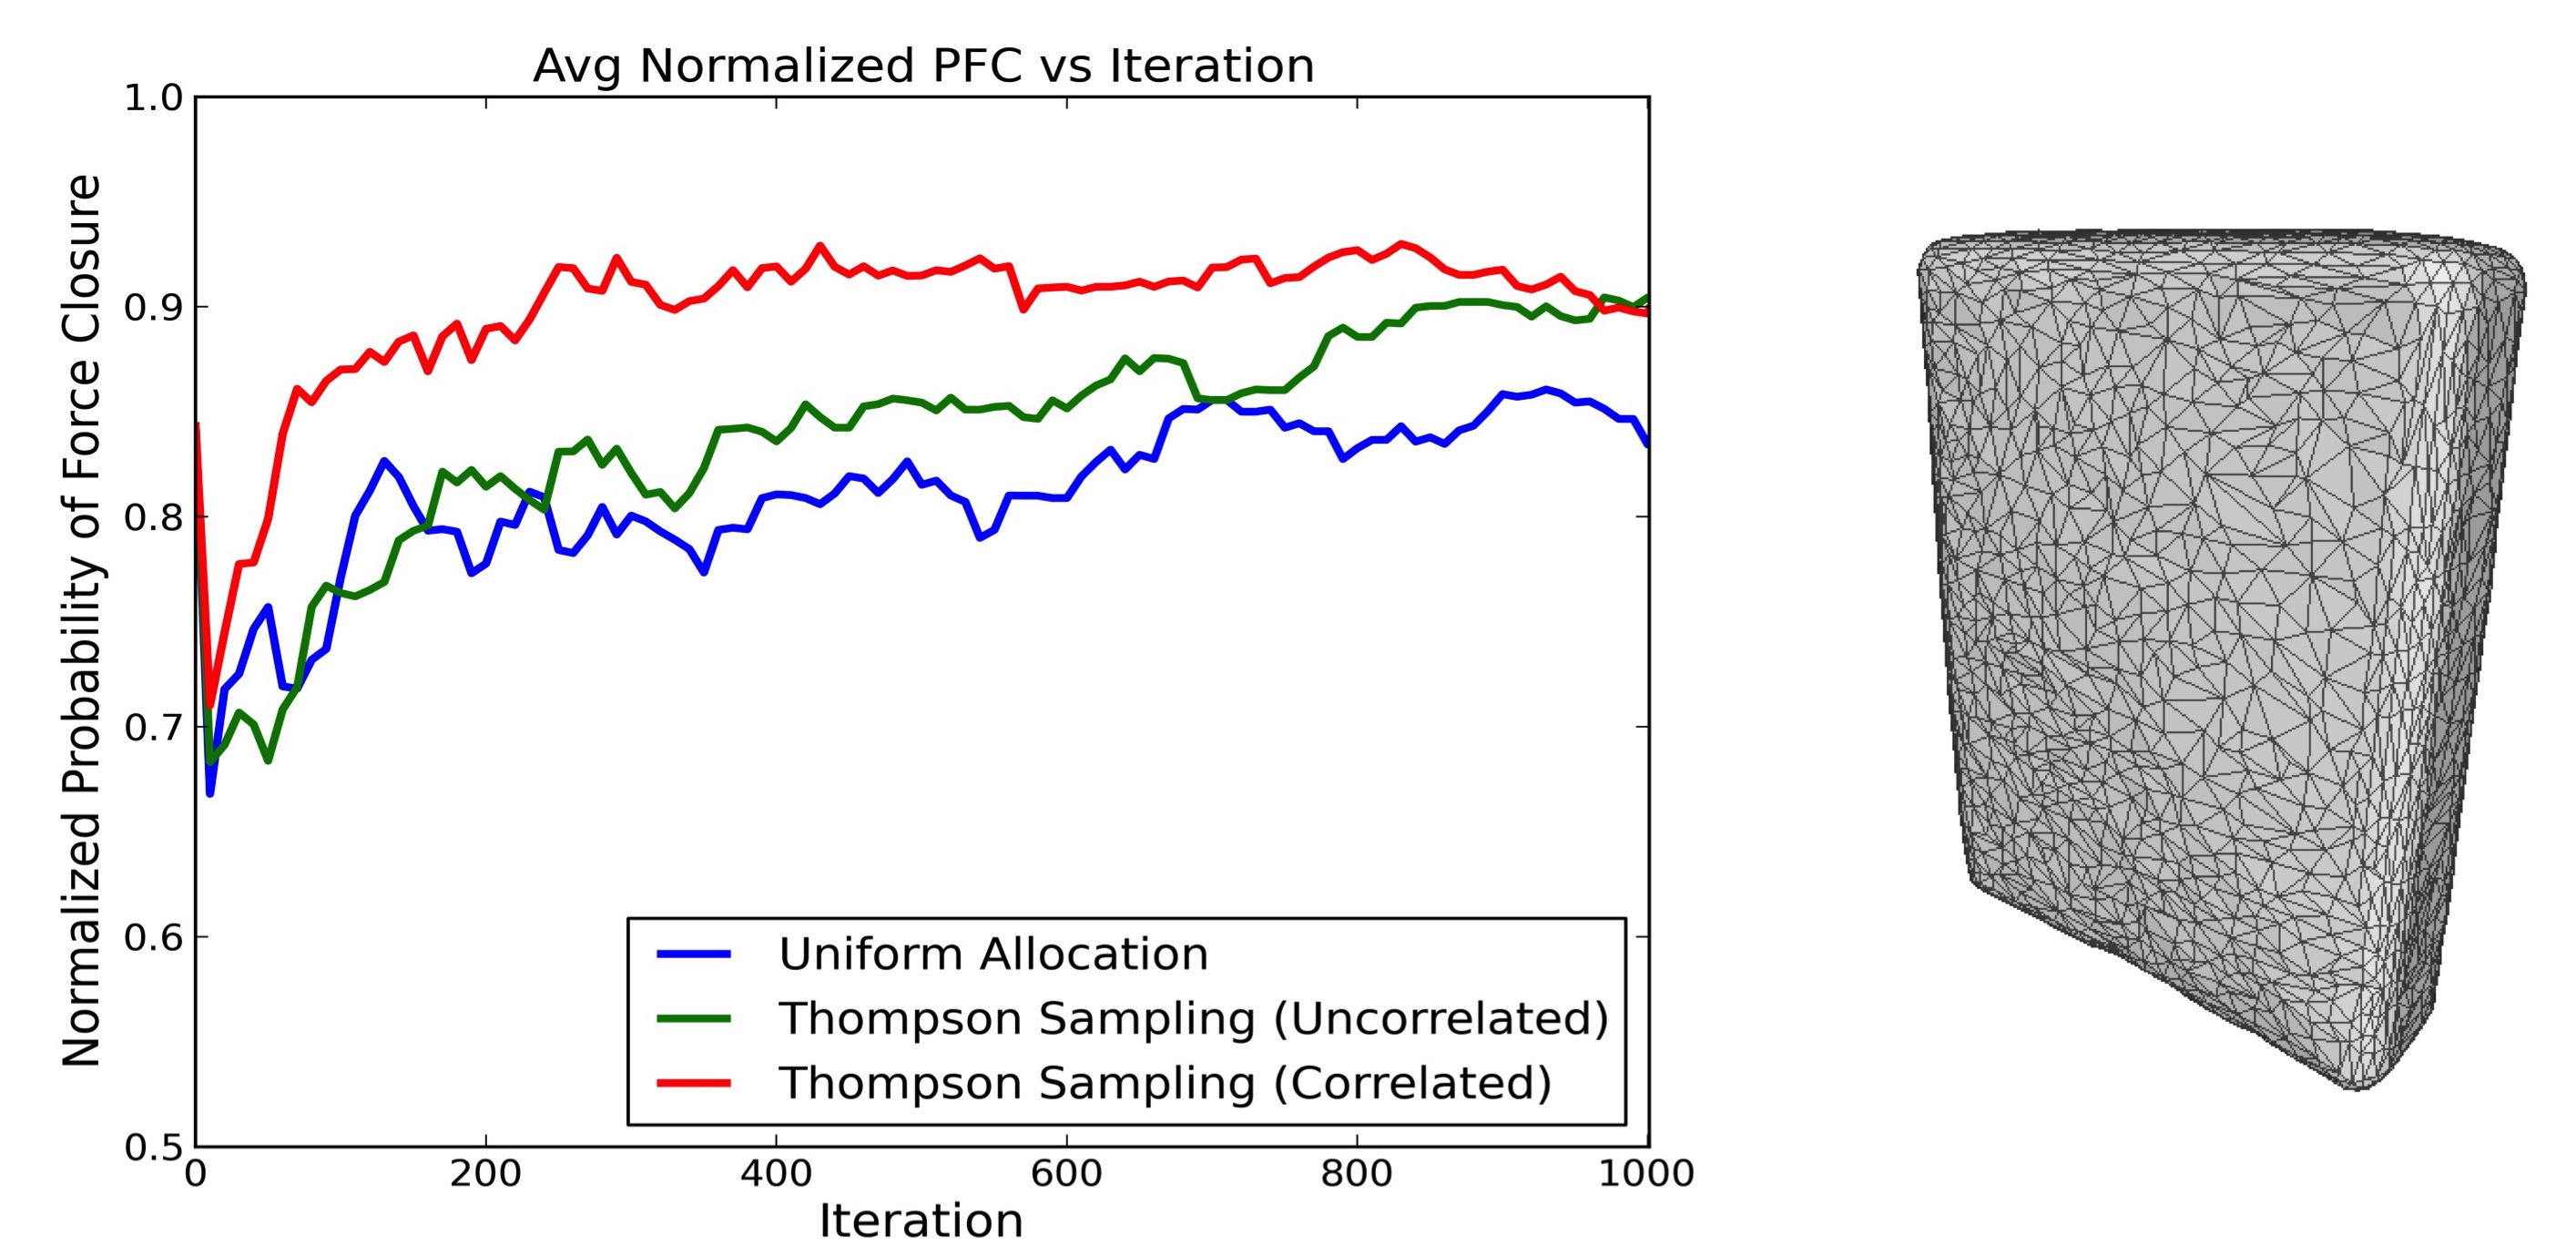
\includegraphics[scale=0.08]{figures/box_avg_reward_w_model.jpg}
        \caption{Normalized $P_F$ on a cereal box with 250 candidate grasps.}
    \end{subfigure}
    \begin{subfigure}[b]{0.5\textwidth}
        \centering
        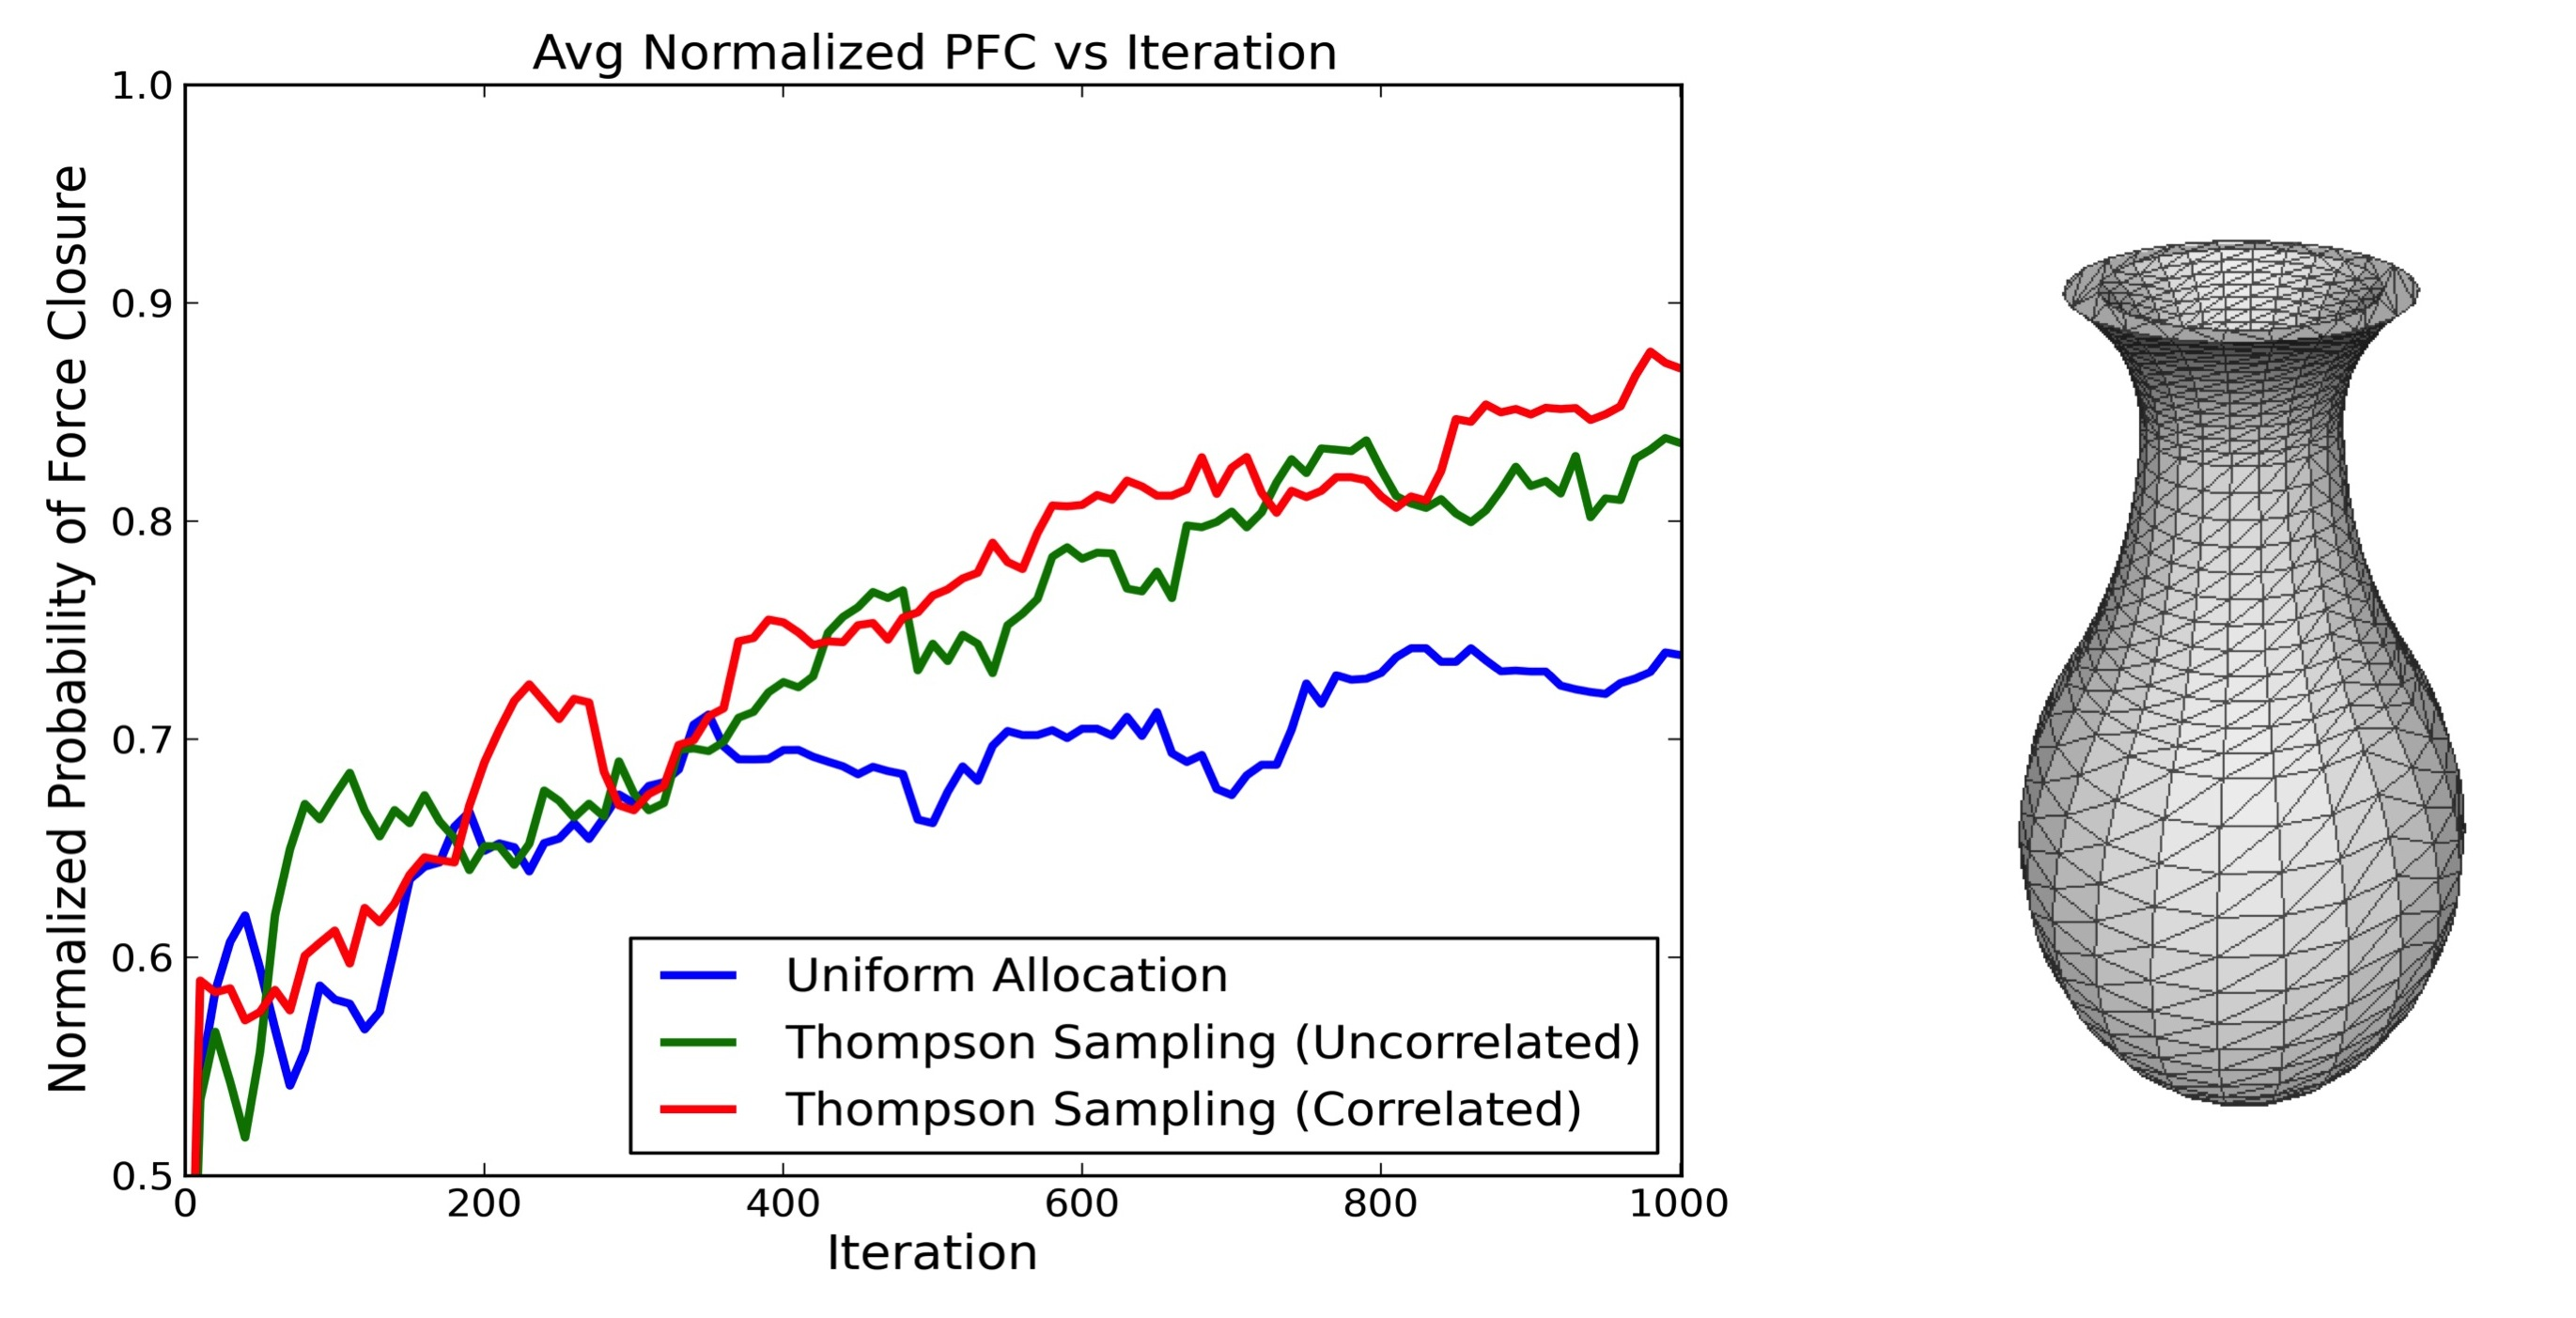
\includegraphics[scale=0.08]{figures/flowerpot_avg_reward_w_model.jpg}
        \caption{Normalized $P_F$ on a flower pot with 250 candidate grasps.}
    \end{subfigure}
\caption{Comparison of the normalized $P_F$ of the sampled grasp versus iteration of the MAB algorithm for correlated Thompson sampling, uncorrelated Thompson sampling, and Uniform Allocation averaged over 20 trials. (a) On the cereal box, correlated Thompson sampling converges to within 90\% of the highest quality grasp approximately 4$\times$ faster than uncorrelated. (b) However, correlated and uncorrelated Thompson sampling perform comparably on the flower pot because there are few grasp similarities in the candidate set. }
\figlabel{local-mab}
\vspace*{-15pt}
\end{figure}

To examine the effects of orders of magnitude of prior data in the MAB algorithms, we ran the algorithms with priors computed from increasingly larger subsets of prior data from DexNet: 0, 15, 150, and 1500 objects. 
\figref{global-mab} shows the normalized probability of force closure $P_F$ versus iteration when planning grasps for a bottle using prior grasp data from the five nearest neighbor objects in DexNet averaged over 50 trials.
Each other object was labelled with 250 grasps and $P_F$ evaluated using brute force Monte-Carlo integration.
We see that the convergence of the correlated MAB algorithms to a grasp with high $P_F$ accelerates with increasingly largers subsets of prior data used.
This suggests that adding more prior data may further accelerate convergence, because it is increasingly likely that a similar object and grasp exists in the dataset as the size increases.
Future work will examine these effects on a larger subset of objects and will use more than five nearest neighbors from DexNet to compute priors, which may lead to even larger gains for larger subsets of prior data.

\begin{figure}[t!]
\centering
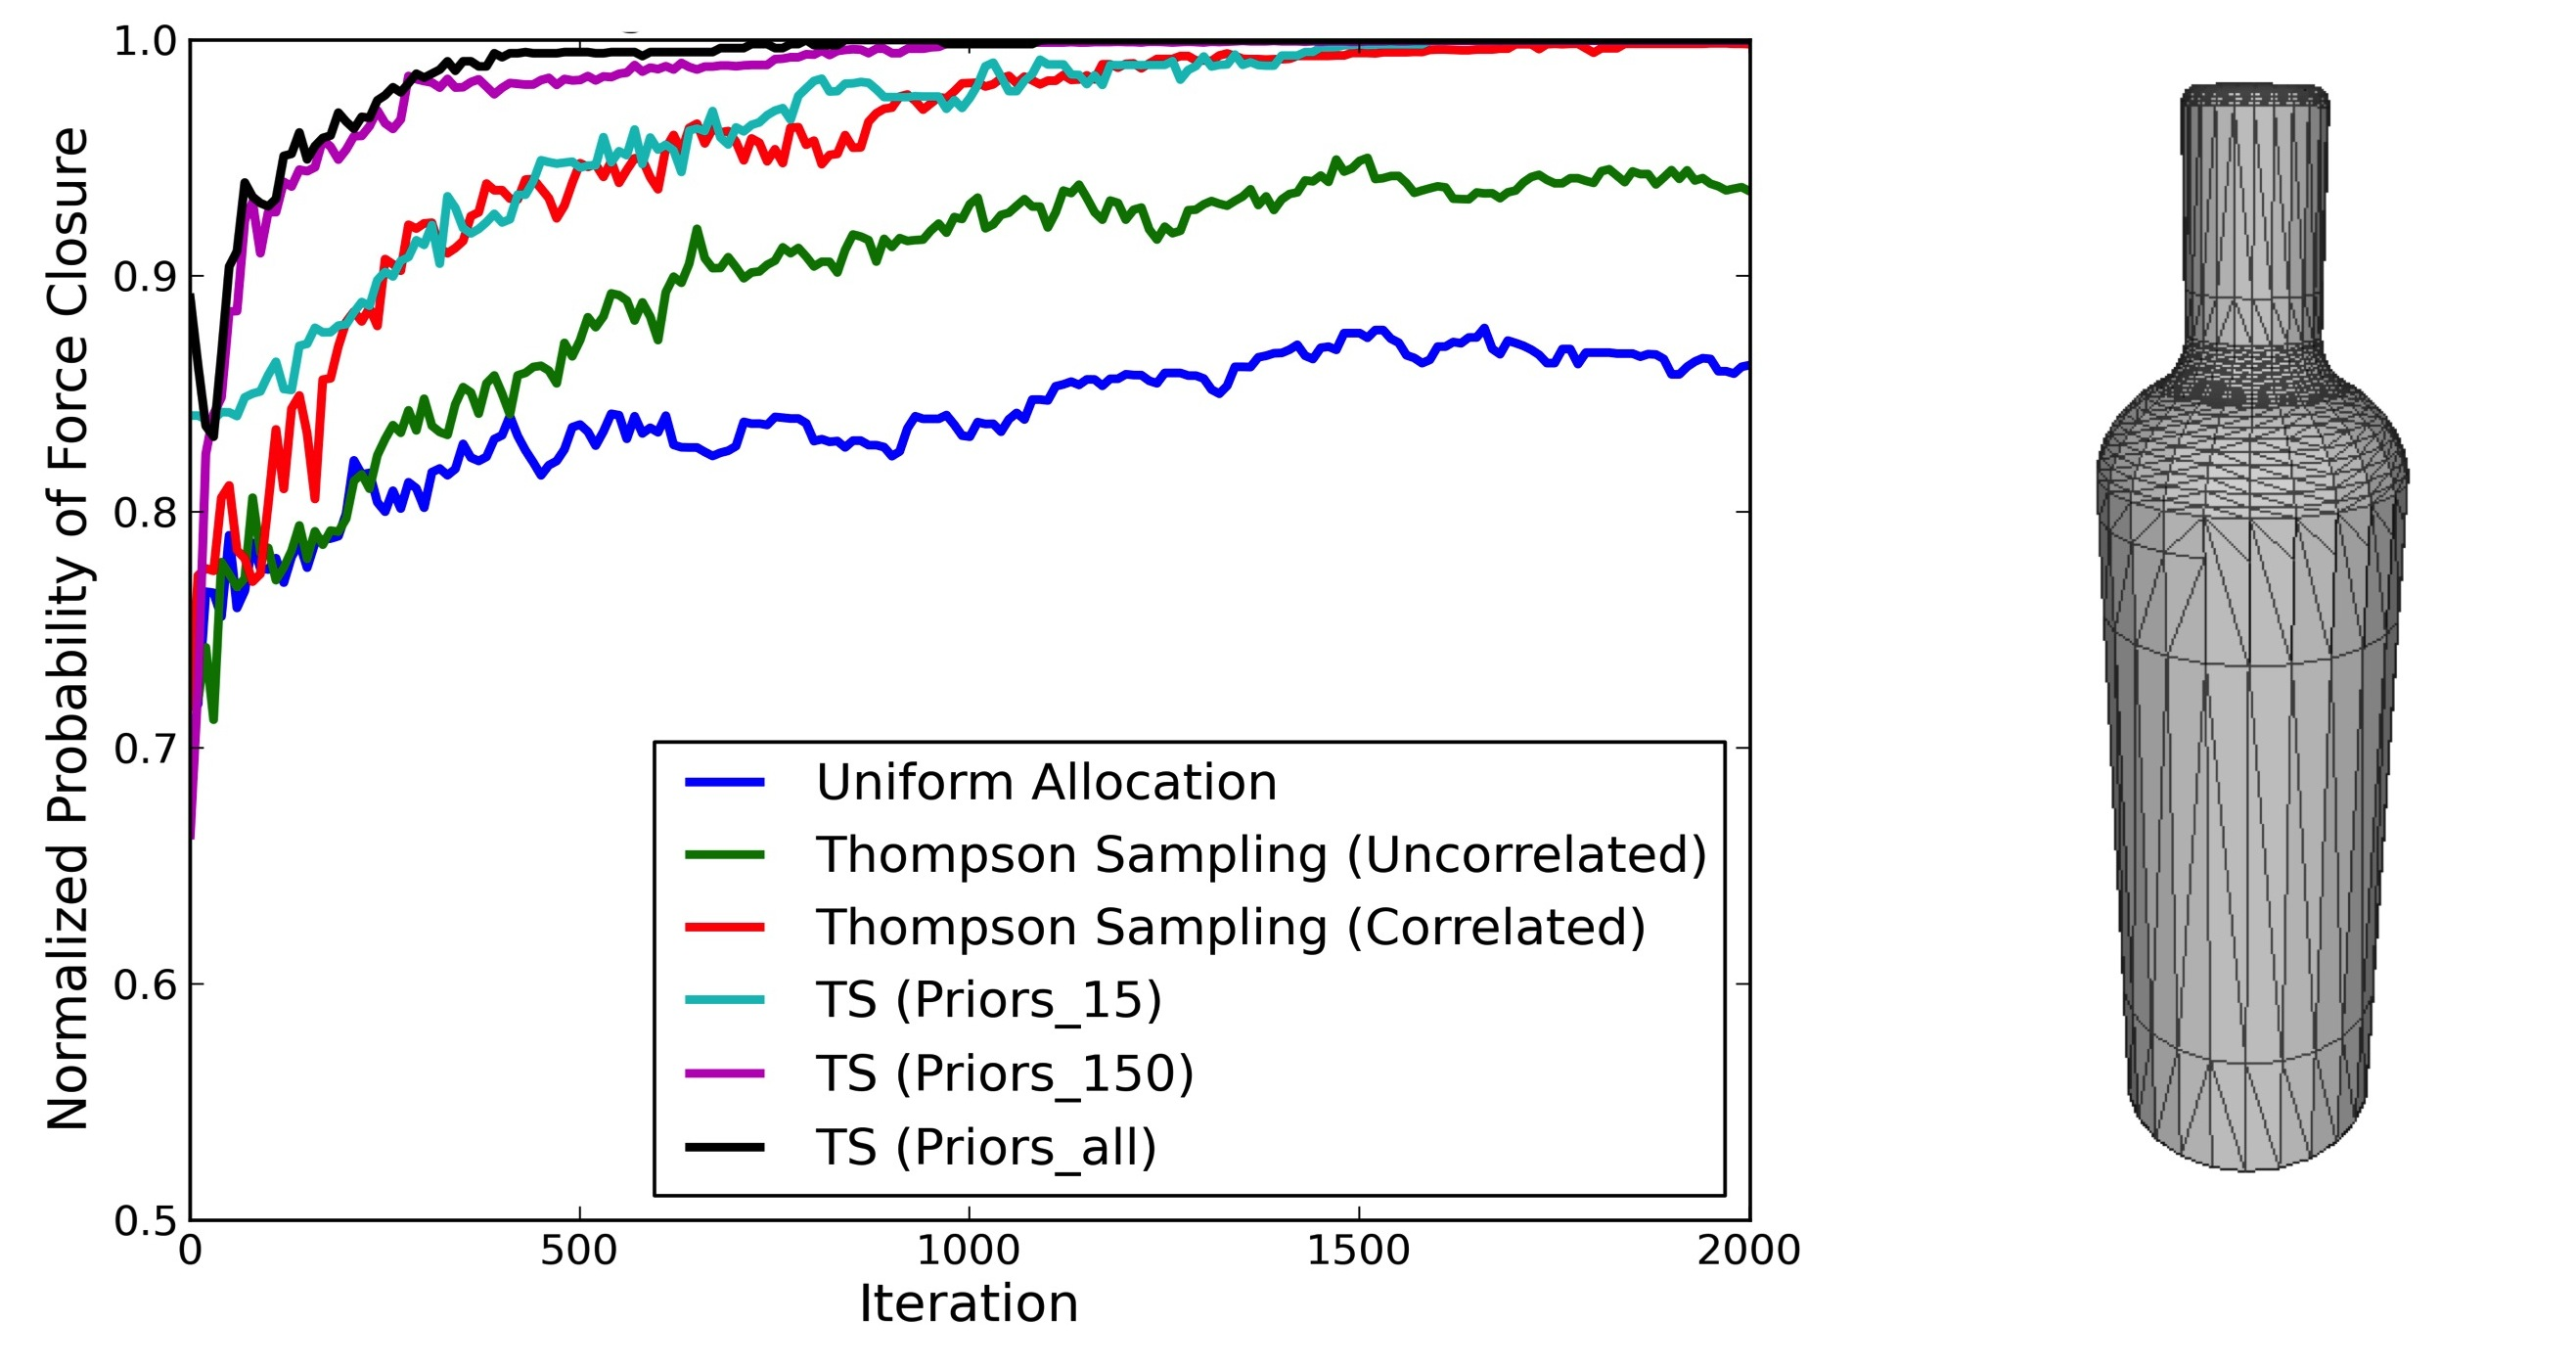
\includegraphics[scale=0.09]{figures/bottle_avg_reward_w_model2.jpg}
\caption{Comparison of the normalized $P_F$ of the sampled grasp (y-axis) versus iteration of the MAB algorithm (x-axis) for correlated Thompson sampling with and without the use of prior grasps from five nearest neighbors from DexNet, uncorrelated Thompson sampling, and Uniform Allocation averaged over 20 trials on the bottle object. Prior grasps were taken from increasingly larger subsets of DexNet: 15, 150, and 1500 objects. We see that convergence to within 90\% of the optimal grasp is accelerated by approximately 10$\times$ over uncorrelated Thompson sampling, and performance appears to improve with increasing sizes of the prior dataset used. }
\figlabel{global-mab}
\vspace*{-15pt}
\end{figure}

We are currently working on an experiment to quantify the gains in convergence time across orders of magnitudes of prior data (10, 100, 1000, 10000) from DexNet using Google Compute Engine.
Our initial version will be run on a relatively small subset of test objects, and in the coming weeks we will average the performance over a larger set of test objects.
We are particularly interested in seeing if there is a point of diminshing returns from adding more data when using datasets on the order of 10,000 - 100,000 objects.
We are also interested in whether or not adding perturbations to the data such as object reflections and shape perturbations will also increase performance, as has been observed for training Deep CNNs in vision~\cite{krizhevsky2012imagenet}.










